\chapter*{Wprowadzenie}
Gry wideo, które dotychczas kojarzone były niemal wyłącznie z pojęciem interaktywnej formy dostarczania rozrywki, od wielu lat zdobywają coraz to nowsze pola zastosowań. Przykładem tutaj mogą być gry oparte o zasadę tzw. \emph{edutainment} (w~tłum. \emph{edurozrywka})\footnote{przykładowy serwis z grami edukacyjnymi - http://www.edugames.pl/}. Mają one na celu efektywne przekazywanie wiedzy, dzięki swojemu atrakcyjnemu i rozrywkowemu charakterowi, w takich dyscypliach naukowych jak biologia, fizyka, informatyka lub języki obce. 
Innym polem zastosowań elementów gier jest biznes. Coraz częściej można spotkać się z pojęciem \emph{gamefication} (w tłum. \emph{grywalizacji}) miejsca pracy. Określa ono zestaw technik i narzędzi związanych z grami, które pomagają motywować pracowników do lepszego wykonywania powierzonej im pracy. Dzieje się to poprzez nagradzanie najlepszych pracowników wirtualnymi punktami doświadczenia, osiągnięciami oraz umieszczaniem ich wizerunku na szczytach rankingów\footnote{przykładowa aplikacja bazująca na idei grywalizacji - https://dueprops.com/}.
Wreszcie, możemy mieć również do czynienia z~grami symulacyjnymi. Ich celem jest umożliwienie graczom doznawania wrażeń znanych z~rzeczywistości, a których oni bezpośrednio mogą na codzień nie doświadczać. Wśród takich gier można wyróżnić gry, których celem jest szkolenie użytkowników - np. symulatory lotu - oraz te, których głównym celem jest dostarczenie użytkownikom rozrywki - np. symulator prowadzenia sieci pizzerii.

\begin{figure}
\begin{center}
	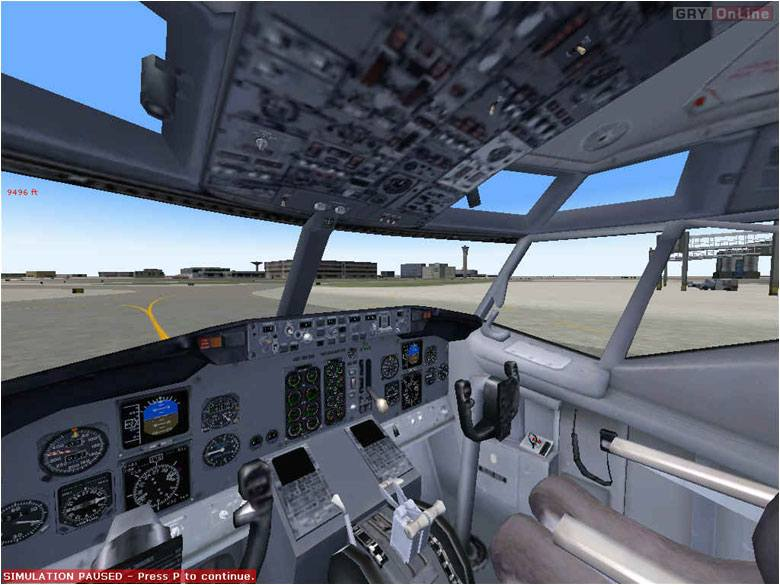
\includegraphics[width=120mm,height=90mm]{images/flightSim}
	\caption{Fligt Simulator 2004 - przykład gry symulacyjnej}
\end{center}
\end{figure}

Niniejsza praca dyplomowa skupia się na projekcie gry symulacyjnej, która odwzorowuje, w dużym uproszczeniu, działania oddziałów antyterrorystyczych podczas szturmu na budynek, zajęty przez wrogie jednostki. Użytkownik grający w tą grę ma możliwość stworzenia schematu budynku, parametryzacji liczby jednostek po obu stronach konfliktu oraz określenia planu działania antyterrorystów. Na podstawie tej konfiguracji gra przeprowadza symulację szturmu na budynek, którą gracz może obserwować.

Realizacja tego projektu obejmuje zaprojektowanie i zaimplementowanie gry oraz omówienie taktyk stosowanych przez strony konfliktu. Zwrócona jest szczególna uwaga na twórcze wykorzystaie algorytmów sztucznej inteligencji, charakterystycznych dla gier wideo. Uzupełnieniem dokumentu jest przedstawienie technologii i bibliotek, które zostały wykorzystane podczas implementacji.


